\documentclass[11pt,a4paper]{article}

% Packages
\usepackage[utf8]{inputenc}
\usepackage[T1]{fontenc}
\usepackage{amsmath,amssymb,amsthm}
\usepackage{graphicx}
\usepackage{hyperref}
\usepackage{booktabs}
\usepackage{xcolor}
\usepackage[margin=2.5cm]{geometry}
\usepackage[numbers]{natbib}
\usepackage[protrusion=true,expansion=false]{microtype}

% Theorem environments
\newtheorem{theorem}{Theorem}[section]
\newtheorem{lemma}[theorem]{Lemma}
\newtheorem{proposition}[theorem]{Proposition}
\newtheorem{definition}[theorem]{Definition}

% Shortcuts
\newcommand{\mc}{\mu_c}
\newcommand{\Neff}{N_{\text{eff}}}
\newcommand{\Ssolve}{S_{\text{solve}}}
\newcommand{\Pfound}{P(\text{found})}
\newcommand{\PSAT}{P(\text{SAT})}
\newcommand{\PfSAT}{P(\text{found}\mid\text{SAT})}

% Title
\title{Predicting Computational Cost from the Structural Parameter~$\delta$:\\
Separating Existence from Discovery in Random 3-SAT}
\author{Akihito Sunagawa\thanks{akihito.sunagawa@gmail.com}}
\date{March 2026}

\begin{document}

\maketitle

\begin{abstract}
Whether a solution \emph{exists} and whether an algorithm can \emph{find} it are
distinct questions governed by different mechanisms.
In random 3-SAT, the first moment method gives
$\PSAT \approx \Neff \cdot e^{-\delta}$,
where $\delta = \alpha n |\!\ln(7/8)|$ is a reparameterization
of the clause density (the exponent in the first moment method).
This characterizes existence but says nothing about discovery.

We introduce the computational budget~$\mu$ (solver operations) and ask:
can the conditional success probability $\PfSAT$ be
multiplicatively decomposed as a function of $\mu / \mc(\delta)$?

Experiments with three solver families (CDCL, WalkSAT, random search)
on instances with $n = 100$--$300$ variables and $\alpha = 3.0$--$4.0$
yield three findings.
(1)~The median runtime scales as $\mc \propto e^{c\delta}$, where the
\emph{sensitivity exponent}~$c$ is solver-dependent:
$c \approx 0.24$ for CDCL,
$c \approx 0.21$ for WalkSAT, and
$c = 1.0$ for random search (exact),
in the floor-free regime $\alpha \geq 3.5$
(fits including $\alpha = 3.0$, where solver startup
overhead dominates, give $c = 0.25$ and $0.18$ respectively;
see Section~\ref{sec:mu_c}).
(2)~The ratio $\mu/\mc$ is an effective normalizing variable:
both solvers exhibit a monotone transition near $\mu/\mc = 1$
with $x_0 \approx 0$, though transition shapes differ by 14--15\%
(model-independent across sigmoid and Weibull fits).
(3)~The ordering $c_{\text{CDCL}} > c_{\text{WalkSAT}}$ is robust
across problem sizes ($n = 100$--$300$), though both estimates
show moderate $n$-dependence (range ${\sim}18\%$ for CDCL,
${\sim}7\%$ for WalkSAT) when measured at a common clause density
range ($\alpha = 3.5$--$4.0$).
A cross-$n$ prediction test (train on $n \leq 200$,
predict $n = 300$) achieves factor-of-2 accuracy
(RMSE $= 0.73$ in log space) over a range where~$\mc$
spans three orders of magnitude
(Appendix~\ref{app:prediction}).

The parameter~$\delta$ thus governs both existence ($c=1$, mathematical identity)
and discovery ($c < 1$, algorithm-dependent), but with qualitatively different
sensitivity.
Notably, $c$ measures sensitivity to~$\delta$, not efficiency:
WalkSAT has the smallest~$c$ yet the largest absolute cost,
because low sensitivity can arise from ignoring structure
rather than exploiting it.

\medskip
\noindent\textbf{Keywords:} random 3-SAT, computational budget,
existence--discovery separation, first moment method,
solver comparison, sensitivity exponent
\end{abstract}

%=============================================
\section{Introduction}
\label{sec:intro}

The satisfiability threshold of random $k$-SAT is among the most studied
phenomena in combinatorics and statistical physics~\cite{MPZ2009}.
The cavity method and its rigorous counterparts determine, with increasing
precision, the critical clause density $\alpha_c$ at which solutions
cease to exist~\cite{Achlioptas2008,Ding2015}.
These results answer the \emph{existence} question:
for a given clause-to-variable ratio~$\alpha$, does a satisfying
assignment exist with high probability?

A complementary question receives far less formal attention:
given that a solution \emph{exists}, how much computation is needed
to \emph{find} it?
Worst-case complexity theory provides upper bounds
(e.g., Sch\"oning's $(2(1-1/k))^n$ for $k$-SAT~\cite{Schoening1999}),
and empirical studies document heavy-tailed runtime
distributions (RTDs)~\cite{Gomes2000,Coarfa2003,Hoos1999,Frost1997}.
Cocco and Monasson~\cite{CoccoMonasson2001} analytically derived
the computational cost of DPLL as a function of clause density,
showing that the typical complexity grows exponentially with an
$\alpha$-dependent rate.
RTDs characterize the probability of finding a solution within
a given time budget, and have been used for algorithm selection
and restart policy design~\cite{Hoos1999}.
Yet no framework connects RTDs to the structural parameter~$\delta$
from the first moment method, nor uses $\delta$ to predict how
the median runtime scales across clause densities.

We formalize this gap through a decomposition that is trivial
as an identity but nontrivial as a quantitative program:
\begin{equation}
\label{eq:decomposition}
\Pfound = \underbrace{\PSAT}_{\text{existence}} \;\times\;
          \underbrace{\PfSAT}_{\text{discovery}}.
\end{equation}
The left factor is well characterized by the first moment method.
The right factor---the \emph{discovery probability}---is what we
measure.

Our central finding is that the same structural parameter~$\delta$
(a reparameterization of the clause density~$\alpha$,
equivalent to the exponent in the first moment method)
governs both factors, but with different strength:
\begin{itemize}
\item \textbf{Existence:} $\PSAT \approx \Neff \cdot e^{-\delta}$
      with $c = 1$ (mathematical identity).
\item \textbf{Discovery:} The median computational cost scales as
      $\mc \propto e^{c\delta}$ with $c < 1$, where $c$ depends
      on the solver family.
\end{itemize}
The sensitivity exponent~$c$ measures how strongly the solver's
cost responds to increasing structural complexity~$\delta$.
It is \emph{not} an efficiency measure:
CDCL ($c \approx 0.24$) is more sensitive to~$\delta$ than
WalkSAT ($c \approx 0.21$), yet CDCL is 10--50$\times$ faster
in absolute terms.
Sophistication increases sensitivity; it does not reduce it.


%=============================================
\section{Framework}
\label{sec:framework}

\subsection{Existence: the first moment baseline}

Consider a random 3-SAT instance with $n$~variables and
$m = \alpha n$ clauses, each a disjunction of 3 literals
chosen uniformly at random.
A uniformly random assignment satisfies a single clause with
probability $1 - 2^{-k} = 7/8$ for $k=3$.
The expected number of satisfying assignments is
\begin{equation}
\label{eq:first-moment}
\mathbb{E}[\#\text{SAT}] = 2^n \cdot (7/8)^m
  = \exp\!\bigl(n\ln 2 - \delta\bigr),
\end{equation}
where
\begin{equation}
\label{eq:delta}
\delta \;\equiv\; \alpha\, n\, |\!\ln(7/8)|
  \;=\; m \cdot |\!\ln(7/8)|
\end{equation}
is a reparameterization of the clause count~$m$
(equivalently, of the clause density~$\alpha$ at given~$n$),
with $|\!\ln(7/8)| \approx 0.134$~nats per clause.
This is the annealed (replica-symmetric) approximation;
the 20\% gap between the annealed threshold
$\alpha_c^{(1)} \approx 5.19$ and the true threshold
$\alpha_c \approx 4.27$~\cite{MPZ2009} reflects replica symmetry
breaking corrections that are well understood but irrelevant
to our purpose.

Equation~\eqref{eq:first-moment} is a mathematical identity
within the annealed framework.
The parameter~$\delta$ is \emph{not} a new quantity:
it is simply $m \cdot |\!\ln(7/8)|$, computable from the instance
specification and identical to the exponent in the first moment
method~\cite{MPZ2009}.
What is new is the empirical observation that $\delta$ also
governs \emph{computational cost}, with a solver-dependent
proportionality constant (Section~\ref{sec:mu_c}).

\subsection{Discovery: introducing the computational budget}

Let $\mu$ denote the computational budget available to a solver
(measured in solver-specific units: conflicts for CDCL, flips for
WalkSAT, random trials for random search).
We define the \textbf{discovery probability}
\begin{equation}
\label{eq:ssolve}
\Ssolve(\delta, \mu) \;\equiv\; \PfSAT
\end{equation}
as the probability that the solver finds a satisfying assignment
within budget~$\mu$, conditioned on the instance being satisfiable.
This is the CDF of the runtime distribution
(RTD)~\cite{Hoos1999,Frost1997}, restricted to satisfiable instances.

Our hypothesis is that $\Ssolve$ admits a
\textbf{multiplicative separation} through the median
runtime~$\mc(\delta)$:
\begin{equation}
\label{eq:separation}
\Ssolve(\delta, \mu) = f\!\left(\frac{\mu}{\mc(\delta)}\right),
\end{equation}
where $f$ is a monotone increasing function (a CDF-like transition)
and the median runtime scales exponentially:
\begin{equation}
\label{eq:mu_c}
\mc(\delta) = A \cdot e^{c\,\delta}.
\end{equation}
Here $c$ is the \textbf{sensitivity exponent}---the rate at which
computational cost grows per unit of~$\delta$---and $A$
is a unit-dependent intercept (absorbing the absolute speed of
the solver implementation).

\paragraph{Why exponential?}
The exponential form in~\eqref{eq:mu_c} is not an arbitrary
modeling choice.
If constraints contribute independently to cost---i.e.,
$\mc(\delta_1 + \delta_2) = \mc(\delta_1) \cdot
[\mc(\delta_2)/A]$---then the Cauchy functional equation
$g(\delta_1 + \delta_2) = g(\delta_1) \cdot g(\delta_2)$
(with $g = \mc/A$, $g(0) = 1$, $g$ continuous and monotone
increasing)
has a unique solution $g(\delta) = e^{c\delta}$ for some
$c > 0$~\cite{Aczel1966}.
In other words, \eqref{eq:mu_c}~is the \emph{only} continuous
scaling law compatible with independent accumulation of
constraints.
The parameter~$c$ is the scale constant of this unique solution,
measuring the solver's intrinsic sensitivity to structural
complexity.
(A formal verification of this characterization theorem in
Lean~4 is available in the supplementary repository.)

\paragraph{Scope of the sensitivity exponent.}
Throughout this paper, $c$ is measured by varying
the clause density~$\alpha$ at \emph{fixed} problem size~$n$.
That is, $\delta$ serves as a reparameterization of~$\alpha$
(at given~$n$) rather than as a universal coordinate mixing
$\alpha$ and~$n$.
This distinction matters because the scaling of runtime
with~$n$ (at fixed~$\alpha$) can differ qualitatively from
the scaling with~$\alpha$ (at fixed~$n$).
In particular, stochastic local search solvers are known
to scale polynomially with~$n$ at the
phase transition~\cite{MuHoos2015},
which is incompatible with treating $\delta = \alpha n|\!\ln(7/8)|$
as a single exponential predictor across both axes.
Section~\ref{sec:asymmetry} discusses this asymmetry in detail.

Crucially, $c$ is invariant under rescaling of~$\mu$:
if $\mu \to k\mu$, then $A \to kA$ but the slope $c$ in
$\ln \mc$ vs.\ $\delta$ is unchanged.
This makes $c$ a property of the \emph{algorithm}, not of
the implementation.

\paragraph{Three testable hypotheses.}
\begin{description}
\item[H1 (Full separation):] $\mc$ is independent of~$\alpha$
  (hence of~$\delta$).
  Different $\alpha$-values would yield the same
  runtime distribution.
\item[H2 ($\mc$-coupled separation):]
  $\mc$ depends on~$\delta$ via Eq.~\eqref{eq:mu_c},
  and $\mu/\mc$ collapses the survival curves across
  different~$\alpha$-values onto a single function~$f$.
\item[H3 (Non-separable):]
  No rescaling of~$\mu$ can collapse curves from
  different~$\alpha$-values.
\end{description}

\paragraph{The $c = 1$ baseline.}
For random search (uniformly sampling assignments and checking),
the expected number of trials to find a solution equals
$2^n / \#\text{SAT} = e^{\delta} / \Neff$.
Hence $\mc^{\text{random}} \propto e^{\delta}$, giving $c = 1$
exactly.
This is not an approximation but a consequence of the first
moment identity~\eqref{eq:first-moment}.
Any solver with $c < 1$ is, in a precise sense, experiencing
less cost growth per unit of structural complexity than
a structureless baseline.


%=============================================
\section{Experimental Setup}
\label{sec:experiments}

\subsection{Instance generation}

We generate random 3-SAT instances with $n \in \{100, 200, 300\}$
variables and clause densities
$\alpha \in \{3.0,\; 3.5,\; 3.86,\; 4.0\}$.
Values $\alpha > 4.2$ are excluded: the fraction of satisfiable
instances drops sharply near the satisfiability
threshold $\alpha_c \approx 4.27$, introducing
\emph{survivor bias}---instances that are found satisfiable
at high~$\alpha$ are systematically easier than typical
satisfiable instances.
For each $(n, \alpha)$ pair, we generate 100--200 instances and
retain only those confirmed satisfiable (by an unlimited CDCL run).

\subsection{Solvers}

Three solver families span a range of algorithmic sophistication:

\begin{description}
\item[CDCL (MiniSat via PySAT):]
  Conflict-driven clause learning~\cite{MarquesSilva1999} with restarts.
  Budget unit: \emph{conflicts} (state transitions in the
  implication graph).
  Budget range: $10^2$--$10^5$.

\item[WalkSAT (pure Python, restart):]
  Stochastic local search~\cite{SKC1994} with noise parameter~$0.5$
  and periodic restarts.
  Budget unit: \emph{flips} (single-variable reassignments).
  Budget range: $10^3$--$10^6$.

\item[Random search:]
  Uniformly random assignment, check all clauses, repeat.
  Budget unit: \emph{trials}.
  Serves as the $c = 1$ theoretical baseline.
\end{description}

\subsection{Measurement protocol}

For each instance, we first run an unlimited solve to obtain
the true runtime (defining $\mc$ as the median over instances
at each~$\alpha$).
We then measure $\Ssolve$ at logarithmically spaced budget
values, recording the fraction of SAT instances solved within
each budget.

The conditional analysis $\PfSAT$ (rather than $\Pfound$)
is essential: at $\alpha = 4.0$, approximately 8\% of instances
are unsatisfiable, and including them would conflate the
existence threshold with the discovery transition.


%=============================================
\section{Results}
\label{sec:results}

\subsection{$\mc \propto e^{c\delta}$: the sensitivity exponent}
\label{sec:mu_c}

Figure~\ref{fig:mu_c} shows $\ln \mc$ versus~$\delta$ for
the three solver families.
Linear regression on the four $\alpha$-values yields:

\begin{figure}[ht]
\centering
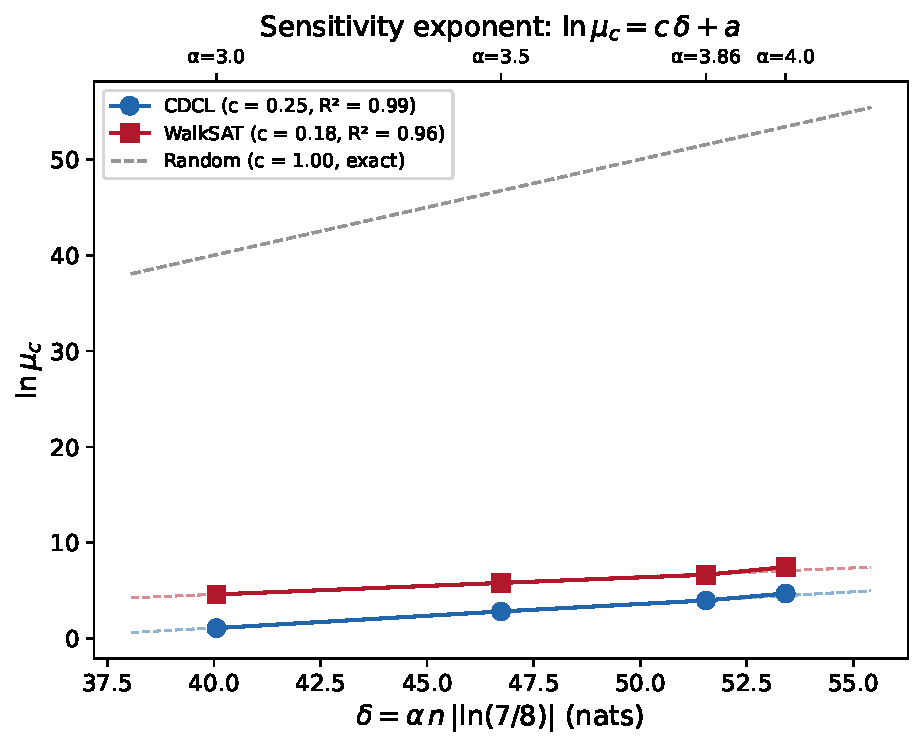
\includegraphics[width=0.85\textwidth]{fig1_sensitivity_exponent.pdf}
\caption{$\ln \mc$ versus~$\delta = \alpha n |\!\ln(7/8)|$
for three solver families ($n = 100$, $\alpha = 3.0$--$4.0$).
Dashed lines: linear fits $\ln \mc = c\delta + a$.
The fit includes $\alpha = 3.0$, where solver startup
overhead creates a floor effect (Section~\ref{sec:discussion});
restricting to $\alpha \geq 3.5$ gives $c \approx 0.24$ (CDCL)
and $c \approx 0.21$ (WalkSAT).}
\label{fig:mu_c}
\end{figure}

\begin{table}[h]
\centering
\begin{tabular}{lcccc}
\toprule
Solver & $c$ & 95\% CI & $R^2$ & Note \\
\midrule
CDCL (conflicts)   & 0.25  & $[0.24,\; 0.29]$ & 0.99  & \\
WalkSAT (flips)    & 0.18  & $[0.17,\; 0.22]$ & 0.96  & \\
Random (trials)    & 1.0   &  ---              &  ---  & Exact (Eq.~\ref{eq:first-moment}) \\
\bottomrule
\end{tabular}
\caption{Sensitivity exponent $c$ from $\ln \mc = c\delta + a$
($n = 100$, $\alpha = 3.0$--$4.0$).
The 95\% CIs are bootstrap percentile intervals
(200 instances $\times$ 10\,000 resamples).
The CIs do not overlap, confirming that the ordering
$c_{\text{CDCL}} > c_{\text{WalkSAT}}$ is statistically significant.
Note: these estimates include $\alpha = 3.0$,
where a floor effect biases~$c$ (Section~\ref{sec:discussion});
restricting to $\alpha \geq 3.5$ gives $c \approx 0.24$ (CDCL)
and $c \approx 0.21$ (WalkSAT).}
\label{tab:c_values}
\end{table}

The slope $c$ is invariant under unit rescaling
($\mu \to k\mu$ shifts the intercept~$a$ but not the slope),
so the difference between CDCL and WalkSAT is not an artifact of
comparing conflicts with flips.

\paragraph{$n$-dependence of $c$.}
Repeating the $\alpha$-regression at $n = 100$, $200$, and $300$
(Appendix~\ref{app:n_scaling}) reveals that the estimated~$c$
depends on the clause density range.
At $\alpha = 3.0$, the median CDCL conflicts are 3--8 across
all~$n$---dominated by solver startup overhead rather than
exponential scaling.
This \emph{floor effect} biases the linear fit:
including $\alpha = 3.0$ gives $c \approx 0.19$,
while restricting to $\alpha \geq 3.5$ gives $c \approx 0.24$
(see also $c = 0.24$ from the 8-point fine-grained fit
in Appendix~\ref{app:alpha_density}).

When measured at a common clause density range
($\alpha = 3.5$--$4.0$, local slope),
both solvers show moderate $n$-dependence:
CDCL gives $c = 0.26$, $0.22$, $0.24$
and WalkSAT gives $c = 0.21$, $0.21$, $0.20$
at $n = 100$, $200$, $300$ (ranges: 18\% and 7\% respectively).
The ordering $c_{\text{CDCL}} > c_{\text{WalkSAT}}$ holds at
every~$n$ tested, with non-overlapping bootstrap 95\% CIs
at $n \geq 200$ ($P > 0.99$); at $n = 100$ the two-point
floor-free slope has wide CIs and the gap is not significant
($P = 0.76$).
The gap (0.02--0.05) is smaller
than the full-range estimates suggest.
WalkSAT's $n$-dependence additionally reflects polynomial
$n$-scaling that the linear-in-$\delta$ model cannot absorb
into the intercept alone
(see Section~\ref{sec:asymmetry} and Appendix~\ref{app:n_scaling}).

\paragraph{Interpretation.}
The ordering $c_{\text{WalkSAT}} < c_{\text{CDCL}} < c_{\text{Random}}$
is initially surprising: the most efficient solver (CDCL) has a
\emph{higher} sensitivity to~$\delta$ than WalkSAT.
This reflects two qualitatively different mechanisms for $c < 1$:
\begin{itemize}
\item CDCL ($c \approx 0.24$): Clause learning actively exploits the
  constraint structure, increasing both efficiency \emph{and}
  sensitivity to that structure.
\item WalkSAT ($c \approx 0.21$): Local search largely ignores global
  constraint structure, making it less responsive
  to~$\delta$---but also less efficient in absolute terms
  ($\mc$ is 10--50$\times$ larger than CDCL).
\end{itemize}
Thus $c$ and absolute efficiency ($1/A$) are independent axes:
$c$ measures \emph{how much} the cost grows with~$\delta$,
while $A$ measures the baseline cost at $\delta = 0$.


\subsection{$\mu/\mc$ as a normalizing variable}
\label{sec:normalization}

Figure~\ref{fig:transition} shows $\Ssolve$ as a function of
$\ln(\mu/\mc)$ for CDCL and WalkSAT across four $\alpha$-values.

\begin{figure}[ht]
\centering
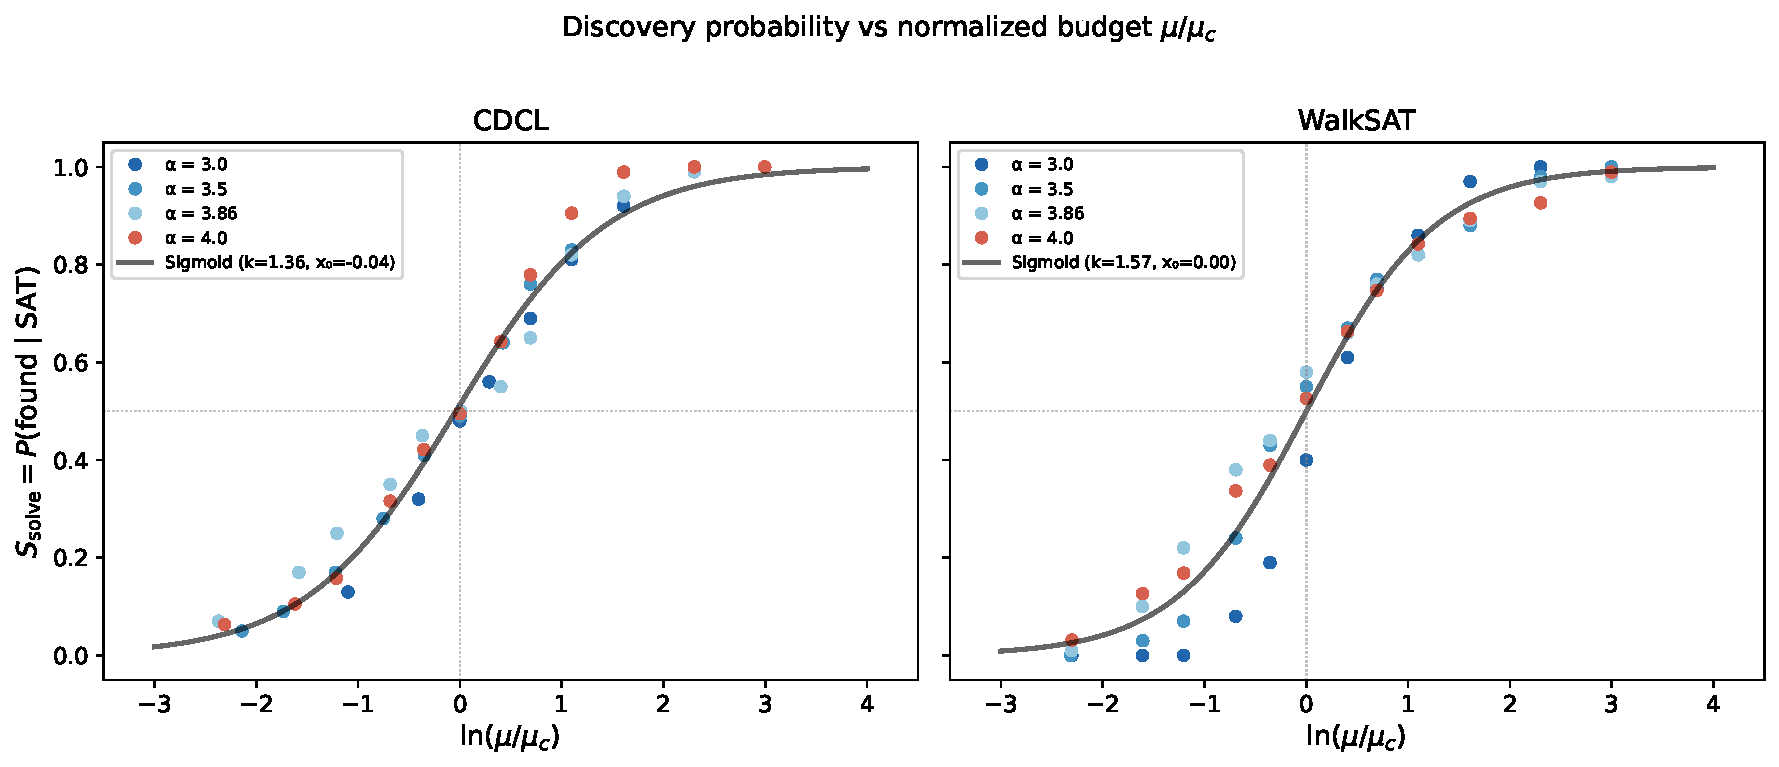
\includegraphics[width=\textwidth]{fig2_transition_curves.pdf}
\caption{Discovery probability $\Ssolve$ versus $\ln(\mu/\mc)$
for CDCL (left) and WalkSAT (right), across four $\alpha$-values
($n = 100$).
Solid curves: sigmoid fits.
Both solvers transition near $\mu/\mc = 1$ ($x_0 \approx 0$),
validating $\mc$ as a natural budget scale.
The steepness~$k$ differs by 14\%
(CDCL: 1.36, WalkSAT: 1.57).}
\label{fig:transition}
\end{figure}

Fitting a logistic (sigmoid) model
$\Ssolve = [1 + \exp(-k(\ln(\mu/\mc) - x_0))]^{-1}$
yields:

\begin{table}[h]
\centering
\begin{tabular}{lcccc}
\toprule
Fit & $k$ & $x_0$ & $R^2$ & $n_{\text{pts}}$ \\
\midrule
CDCL only     & 1.36 & $-0.04$ & 0.985 & 45 \\
WalkSAT only  & 1.57 & $ 0.00$ & 0.972 & 48 \\
Combined      & 1.46 & $-0.01$ & 0.976 & 93 \\
\bottomrule
\end{tabular}
\caption{Sigmoid fit parameters for the transition curves.
Both solvers have $x_0 \approx 0$, confirming that $\mc$ (the median
runtime) naturally marks the 50\% transition point.
The steepness~$k$ differs by 14\%.}
\label{tab:sigmoid}
\end{table}

Two key observations:
\begin{enumerate}
\item Both solvers have $x_0 \approx 0$, meaning the 50\%
  success probability occurs near $\mu = \mc$.
  This validates the median runtime as a natural scale
  for the computational budget.
\item The steepness parameter~$k$ differs by 14\%
  (CDCL: 1.36, WalkSAT: 1.57).
  We do \emph{not} claim a universal scaling function;
  instead, we report that $\mu/\mc$ is an effective normalizing
  variable whose transition shape retains solver-specific features.
\end{enumerate}

At $\mu/\mc = 1.0$, CDCL achieves $\Ssolve = 0.48$--$0.50$
across all four $\alpha$-values (nearly perfect collapse),
while WalkSAT shows $\Ssolve = 0.40$--$0.58$ (more scatter).
This suggests that conflicts are a more natural unit for~$\mu$
than flips.

\paragraph{Model independence.}
To verify that the 14\% shape difference is not an artifact
of the sigmoid functional form, we also fit a Weibull CDF
$\Ssolve = 1 - \exp(-(\mu/\mc)^\beta)$.
The Weibull shape parameter shows a comparable 15\% difference
between solvers (Table~\ref{tab:weibull} in Appendix~\ref{app:model}).
AIC comparison reveals that the best-fit model itself is
solver-dependent: Weibull ($\beta = 0.93$) for CDCL,
sigmoid for WalkSAT.
The shape difference is therefore a genuine property of
the runtime distributions, not a fitting artifact.


\subsection{Runtime heterogeneity}
\label{sec:heterogeneity}

The Weibull shape parameter~$\beta$ provides insight into
runtime distribution structure:

\begin{table}[h]
\centering
\begin{tabular}{lccc}
\toprule
Solver & $c$ & Weibull $\beta$ & $\Delta\beta$ (vs Random) \\
\midrule
Random   & 1.00 & $0.87 \pm 0.05$ & baseline \\
CDCL     & 0.25 & 0.93 & $+0.06$ \\
WalkSAT  & 0.18 & 1.10 & $+0.23$ \\
\bottomrule
\end{tabular}
\caption{Weibull shape parameter by solver.
$\beta < 1$ for random search reflects inter-instance
heterogeneity (a known property of exponential mixtures).
$\Delta\beta$ measures how much each solver homogenizes
instance difficulty.}
\label{tab:beta}
\end{table}

The random search baseline $\beta = 0.87 < 1$ is not anomalous:
it is the expected signature of a mixture of exponential
distributions with varying success probabilities across instances
(the decreasing hazard rate property of mixtures).
Each solver's $\Delta\beta$ relative to this baseline
measures the degree to which the algorithm \emph{homogenizes}
instance difficulty.

Note that $c$ and $\beta$ are not monotonically related
($c$: Random $>$ CDCL $>$ WalkSAT;
$\beta$: WalkSAT $>$ CDCL $>$ Random):
they measure different aspects of the solver--structure interaction.
Sensitivity~$c$ captures how cost \emph{scales} with~$\delta$;
$\Delta\beta$ captures how much the solver \emph{equalizes}
instances of varying difficulty.


%=============================================
\section{Discussion}
\label{sec:discussion}

\subsection{The sensitivity exponent $c$}

The exponent $c$ in $\mc \propto e^{c\delta}$ measures
the algorithm's \emph{sensitivity} to the clause density
reparameterization~$\delta$.
The theoretical upper bound is $c = 1$ (random search),
since no algorithm can have its cost grow faster with~$\delta$
than the solution density shrinks.

The observation $c_{\text{WalkSAT}} < c_{\text{CDCL}}$ is instructive.
One might expect that a more sophisticated algorithm would have
lower~$c$, interpreting small~$c$ as ``more efficient.''
The data refute this: CDCL is faster by 10--50$\times$
yet \emph{more} sensitive to~$\delta$.
This is because CDCL's clause learning mechanism
\emph{directly engages} with the constraint structure---conflict-driven
learning reads and responds to~$\delta$, making CDCL's cost
track structural complexity more closely.
WalkSAT's local search, by contrast, operates with minimal
awareness of global structure, resulting in lower sensitivity
but higher absolute cost.

Thus $c$ and absolute efficiency ($1/A$ in Eq.~\ref{eq:mu_c})
constitute two independent axes of algorithmic characterization:
\begin{itemize}
\item $c$ (slope): how much does $\delta$ amplify the cost?
\item $1/A$ (intercept): how fast is the solver at $\delta = 0$?
\end{itemize}
A complete characterization of a solver's relationship to
problem structure requires both.

\paragraph{Connection to proof complexity.}
The sensitivity exponent~$c$ is related to, but distinct from,
proof complexity measures.
Ben-Sasson and Wigderson~\cite{BenSasson2001} showed that
resolution proof width lower-bounds proof size,
and Pipatsrisawat and Darwiche~\cite{Pipatsrisawat2011}
proved that CDCL with restarts can polynomially simulate
general resolution.
These results characterize \emph{worst-case} proof length;
$c$ instead captures how the \emph{typical} runtime scales
with~$\delta$, a distributional rather than worst-case measure.
The analytical DPLL results of Cocco and
Monasson~\cite{CoccoMonasson2001} are closer in spirit:
their $\alpha$-dependent exponential rate for DPLL corresponds
to a specific value of~$c$ in our framework, though the
relationship is not exact because their analysis assumes
a pure backtracking solver without clause learning.

\subsection{The $\alpha$--$n$ asymmetry}
\label{sec:asymmetry}

The quantity $\delta = \alpha n |\!\ln(7/8)|$ enters symmetrically
in~$\alpha$ and~$n$, but computational cost does not respect
this symmetry.
Mu and Hoos~\cite{MuHoos2015} demonstrated that
SLS-based solvers (WalkSAT/SKC, BalancedZ, probSAT)
scale \emph{polynomially} with~$n$ at the phase transition
($\mu_c \sim n^b$ with $b \approx 3$), while DPLL-based solvers
scale exponentially ($\mu_c \sim 1.03^n$).

If the model $\mc = A \cdot e^{c\delta}$ held uniformly across
both axes, it would predict $\mc \propto e^{c \alpha |\ln(7/8)| \cdot n}$
at fixed~$\alpha$---exponential in~$n$ for any $c > 0$.
For WalkSAT with $c \approx 0.21$ at $\alpha_c \approx 4.27$,
this gives $\mc \propto 1.13^n$, which is incompatible with
the polynomial scaling found by~\cite{MuHoos2015}.

\paragraph{Direct evidence from $n$-scaling experiments.}
Our own WalkSAT experiments at $n = 100$, $200$, and $300$
confirm this incompatibility (Appendix~\ref{app:n_scaling}).
At clause densities where all instances are solved
(no survivor bias), the growth \emph{decelerates} with~$n$:
\begin{center}
\begin{tabular}{lccc}
\toprule
$\alpha$ & $\gamma$ ($\mc \sim n^\gamma$) &
  Deceleration ratio & Character \\
\midrule
3.0 & 1.07 & 0.48 & nearly linear \\
3.5 & 1.69 & 0.75 & polynomial \\
\bottomrule
\end{tabular}
\end{center}
The deceleration ratio (growth rate $n$: 200$\to$300
divided by 100$\to$200) equals 1.0 for exponential
and $< 1$ for polynomial growth; both values are clearly
sub-exponential.
The power-law exponent~$\gamma$ increases with~$\alpha$,
consistent with Mu and Hoos's $\gamma \approx 3.2$ at
$\alpha_c \approx 4.27$.

Meanwhile, the $\alpha$-sensitivity exponent~$c$ itself
shows $n$-dependence for both solvers when measured at
a common clause density range
(Appendix~\ref{app:n_scaling}):
at $\alpha = 3.5$--$4.0$, CDCL gives
$c = 0.26$, $0.22$, $0.24$ (range 18\%)
and WalkSAT gives $c = 0.21$, $0.21$, $0.20$ (range 7\%).
Bootstrap CIs confirm that WalkSAT's~$c$ decreases
significantly from $n = 100$ to $n = 300$
(95\% CIs: $[0.18, 0.29]$ and $[0.11, 0.14]$, non-overlapping),
consistent with polynomial $n$-scaling compressing the
apparent $\alpha$-sensitivity at larger~$n$.
This $n$-dependence is a symptom of the
product structure $\delta = \alpha \cdot n \cdot |\!\ln(7/8)|$
being an imperfect coordinate:
a model that treats $\alpha$ and $n$ symmetrically
cannot fully accommodate the solver-specific $n$-scaling.
For WalkSAT, this is acute: polynomial $n$-scaling
is fundamentally incompatible with the exponential prediction.

\paragraph{Resolution.}
The sensitivity exponent~$c$ characterizes the
\emph{$\alpha$-sensitivity} of computational cost at fixed~$n$,
not a universal scaling law.
The intercept~$A$ in Eq.~\eqref{eq:mu_c} implicitly depends
on~$n$, absorbing the $n$-scaling.
A more complete model takes the form
\[
\ln \mc(\alpha, n) = c \cdot \alpha \, n \, |\!\ln(7/8)| + g(n),
\]
where $g(n)$ captures the $n$-scaling and differs qualitatively
by solver family:
\begin{itemize}
\item \textbf{CDCL:} $g(n) \approx -0.075\,n$ (linear),
  yielding at $\alpha_c \approx 4.27$ an effective growth rate
  $\mc \propto 1.034^n$---consistent with Mu and Hoos's
  $1.03^n$ for DPLL.
  Both directions are exponential, so~$\delta$ functions
  as a valid (if imperfect) unified coordinate.
\item \textbf{WalkSAT:} Polynomial $n$-scaling
  ($\mc \sim n^{\gamma(\alpha)}$)
  requires $g(n) \sim \gamma \ln n
  - c \cdot \alpha \cdot n \cdot |\!\ln(7/8)|$---a term that
  must grow as $-\Theta(n)$ to cancel the exponential prediction.
  The product structure of~$\delta$ fundamentally breaks down,
  and $c$ itself becomes $n$-dependent.
\end{itemize}

This asymmetry reflects the known distinction
between constraint density and search space size:
$\alpha$ controls the former while $n$ controls the latter.
CDCL---which reads the constraint structure via clause
learning---responds exponentially to both;
WalkSAT---which operates locally---responds exponentially
to~$\alpha$ but only polynomially to~$n$.
Accordingly, $\delta$ is best understood as a
reparameterization of~$\alpha$ at fixed~$n$,
not as a universal coordinate over the
$(\alpha, n)$ plane.

\subsection{Limitations and future work}

\paragraph{Problem size and floor effect.}
Our results cover $n = 100$--$300$.
At $\alpha \leq 3.0$, the median CDCL runtime (3--8 conflicts)
is dominated by solver startup overhead, creating a floor
in~$\ln \mc$ that biases the linear fit downward.
The estimated~$c$ consequently depends on the clause density
range: fits including $\alpha = 3.0$ give $c \approx 0.19$,
while fits restricted to $\alpha \geq 3.5$ give $c \approx 0.24$
(consistent with the fine-grained estimate in
Appendix~\ref{app:alpha_density}).
A cross-$n$ prediction test (Appendix~\ref{app:prediction})
achieves factor-of-2 accuracy over three orders of magnitude
in~$\mc$, demonstrating nontrivial predictive power despite
the floor effect.
Extension to $n \geq 500$---where clustering phenomena
become more pronounced~\cite{Achlioptas2008}---remains untested.

\paragraph{Clause density range.}
We restrict to $\alpha \leq 4.0$ to avoid survivor bias.
The behavior of~$c$ near the satisfiability threshold
$\alpha_c \approx 4.27$ remains an open question.
Fine-grained experiments ($\Delta\alpha = 0.05$) show
local slope fluctuations for both solvers, but the signal-to-noise
ratio at $\Delta\delta \approx 4$~nats is insufficient
to resolve systematic $\alpha$-dependence.

\paragraph{Cross-domain analogies.}
The existence--discovery separation and the role of a
sensitivity exponent may extend beyond SAT.
In large language model (LLM) chain reasoning,
externalizing intermediate steps (chain-of-thought) reduces
the effective decay rate from $\alpha \approx 0.6$ to
$\alpha \approx 0$, paralleling how algorithmic sophistication
modifies~$c$ in SAT.
However, the LLM decay rate measures success probability per
chain step, while~$c$ measures cost scaling per unit~$\delta$;
the correspondence is suggestive but not quantitative.
More broadly, extending the $\mc \propto e^{c\delta}$ model
to other domains requires an operational definition of~$\delta$
(the structural constraint parameter) that is independent of
the outcome it predicts---a condition that SAT satisfies
via the first moment method but that is nontrivial elsewhere.


%=============================================
\section{Conclusion}
\label{sec:conclusion}

We have separated the question of solution \emph{existence}
from solution \emph{discovery} in random 3-SAT:
\[
\Pfound = \PSAT \times \PfSAT.
\]
The first factor is governed by the first moment method with $c = 1$.
The second factor---quantified here for the first time---shows
that the median computational cost scales as $\mc \propto e^{c\delta}$
with $c < 1$ for nontrivial algorithms, and that $\mu/\mc$
serves as an effective normalizing variable for the discovery
transition.

The sensitivity exponent~$c$ is solver-dependent
(CDCL: ${\sim}0.24$, WalkSAT: ${\sim}0.21$, Random: 1.0
in the floor-free regime $\alpha \geq 3.5$).
The ordering $c_{\text{CDCL}} > c_{\text{WalkSAT}}$ holds
at all problem sizes tested ($n = 100$--$300$),
though both solvers show moderate $n$-dependence
(CDCL: range 18\%, WalkSAT: range 7\%
at $\alpha = 3.5$--$4.0$).
For CDCL, $\delta$ serves as an effective unified coordinate
for both $\alpha$- and $n$-scaling;
for WalkSAT, $\delta$'s product structure does not extend
to the $n$-direction due to polynomial
$n$-scaling~\cite{MuHoos2015},
and $c$ is best interpreted as an $\alpha$-sensitivity at fixed~$n$.
Across solver families, $c$ captures a property distinct from
efficiency: sophistication \emph{increases} sensitivity to
problem structure ($c_{\text{CDCL}} > c_{\text{WalkSAT}}$),
even as it decreases absolute cost
($A_{\text{CDCL}} \ll A_{\text{WalkSAT}}$).

The same first-moment exponent~$\delta$ that governs
solution existence also predicts how computational cost
scales with clause density---but with a solver-dependent
discount factor~$c < 1$.
Runtime distributions have been extensively studied for algorithm
selection and restart design~\cite{Hoos1999,Frost1997,Gomes2000},
and the first moment method is a standard tool in random CSP
theory~\cite{MPZ2009}.
Our contribution is the quantitative bridge: the same
exponent~$\delta$ from the first moment method predicts
how the \emph{median} of the RTD scales with clause density,
with the solver-dependent discount factor~$c$ as the key
new quantity.


%=============================================
\appendix

\section{$n$-scaling of the sensitivity exponent}
\label{app:n_scaling}
\label{sec:n_scaling}

\paragraph{CDCL.}

\begin{table}[h]
\centering
\begin{tabular}{lcccc}
\toprule
$n$ & $c$ (slope) & Intercept $a$ & $R^2$ & Instances \\
\midrule
100 & 0.184 & $-5.86$  & 0.92 & 100/$\alpha$ \\
200 & 0.194 & $-13.38$ & 0.99 & 100/$\alpha$ \\
300 & 0.191 & $-21.18$ & 0.98 & 200/$\alpha$ \\
\bottomrule
\end{tabular}
\caption{CDCL: Sensitivity exponent $c$ and intercept $a$
(from $\ln \mc = c\delta + a$) across problem sizes.
Note: the $\alpha$-ranges differ by~$n$
($n = 100{,}200$: $\alpha = 3.0$--$4.27$;
$n = 300$: $\alpha = 3.0$--$4.0$),
and $\alpha = 3.0$ falls in the floor regime
(median conflicts 3--8, Section~\ref{sec:discussion}).
The intercept decreases approximately linearly
with~$n$: $\Delta a / \Delta n \approx -0.075$.}
\label{tab:n_scaling}
\end{table}

The intercept $a(n)$ decreases linearly with~$n$, meaning
the full model is
\[
\ln \mc(\alpha, n) \approx c \cdot \alpha\, n\, |\!\ln(7/8)|
  + g(n), \quad g(n) \approx -0.075\, n + 1.6.
\]
At fixed~$\alpha$, the effective exponential growth rate in~$n$
is $c \cdot \alpha \cdot |\!\ln(7/8)| - 0.075$.
At $\alpha = \alpha_c \approx 4.27$:
\[
\text{rate} = 0.19 \times 4.27 \times 0.134 - 0.075
  \approx 0.033,
\]
predicting $\mc \propto 1.034^n$.
(Here $c = 0.19$ and $g(n)$ are paired values from the same
full-range fit; using floor-free $c \approx 0.24$ would require
a correspondingly steeper $g(n)$, yielding a similar net rate.)
This is consistent with Mu and Hoos's~\cite{MuHoos2015}
finding that DPLL-based solvers scale as $\sim\! 1.03^n$.
The negative intercept $g(n)$ thus absorbs most of the
$n$-dependence, reducing the naive prediction from
$1.11^n$ (slope alone) to $1.034^n$ (slope $+$ intercept).

\paragraph{WalkSAT.}

\begin{table}[h]
\centering
\begin{tabular}{lcccc}
\toprule
$n$ & $c$ (slope) & Intercept $a$ & $R^2$ & Instances \\
\midrule
100 & 0.172 & $-2.16$  & 0.98 & 50/$\alpha$ \\
200 & 0.144 & $-6.18$  & 0.95 & 50/$\alpha$ \\
300 & 0.143 & $-11.62$ & 0.95 & 50/$\alpha$ \\
\bottomrule
\end{tabular}
\caption{WalkSAT: Sensitivity exponent $c$ and intercept $a$
across problem sizes (full-range fit including $\alpha = 3.0$).
The slope~$c$ decreases with~$n$
(range 18.9\%, mean $\bar{c} = 0.153$).
At a common clause density range ($\alpha = 3.5$--$4.0$,
local slope), the $n$-dependence is smaller:
$c = 0.21$, $0.21$, $0.20$ (range 7\%).}
\label{tab:n_scaling_ws}
\end{table}

At clause densities with no survivor bias
($\alpha = 3.0$, $3.5$; solve rate $= 1.0$ at all~$n$),
the median runtime grows as a power law in~$n$:

\begin{table}[h]
\centering
\begin{tabular}{lrrrccc}
\toprule
$\alpha$ & $\mc$(100) & $\mc$(200) & $\mc$(300)
  & $\gamma$ & Decel.\ ratio \\
\midrule
3.0 & 124 & 274 & 402 & 1.07 & 0.48 \\
3.5 & 288 & 836 & 1{,}846 & 1.69 & 0.75 \\
\bottomrule
\end{tabular}
\caption{WalkSAT median flips at bias-free clause densities.
The power-law exponent $\gamma$ (from $\mc \sim n^\gamma$)
and the deceleration ratio
(= growth 200$\to$300 / growth 100$\to$200; equals 1.0 for
exponential, $< 1$ for polynomial) both confirm sub-exponential
$n$-scaling.}
\label{tab:n_scaling_ws_raw}
\end{table}

The deceleration ratio is clearly below~1 at both clause densities,
ruling out exponential $n$-scaling.
The increasing $\gamma$ with~$\alpha$ is consistent with
Mu and Hoos's~\cite{MuHoos2015} finding of
$\gamma \approx 3.2$ at $\alpha_c \approx 4.27$.
Higher clause densities ($\alpha = 3.86$, $4.0$) show
accelerating growth at $n = 300$, but with solve rates of
$0.84$ and $0.60$ respectively, survivor bias makes these
estimates unreliable.

Together, the CDCL and WalkSAT data confirm that
$\delta = \alpha \cdot n \cdot |\!\ln(7/8)|$ serves as
a valid unified coordinate only for solvers whose
$n$-scaling is also exponential (CDCL).
For polynomial-$n$ solvers (WalkSAT), $c$ remains a useful
measure of $\alpha$-sensitivity at fixed~$n$, but the
product structure of~$\delta$ does not extend to the
$n$-direction.


\section{Cross-$n$ prediction test}
\label{app:prediction}

To test whether the model $\ln \mc = c\delta + g(n)$ has
\emph{predictive} (not merely descriptive) power,
we train a pooled regression
$\ln \mc = c\,\delta + b\,n + a_0$
on data at $n = 100$ and $n = 200$
(common $\alpha = 3.0$, $3.5$, $4.0$;
6~training points per solver)
and predict $\mc$ at $n = 300$.

\begin{table}[h]
\centering
\begin{tabular}{lrrrc}
\toprule
$\alpha$ & $\mc^{\text{pred}}$ & $\mc^{\text{actual}}$
  & Ratio & $|\Delta\ln\mc|$ \\
\midrule
\multicolumn{5}{l}{\textit{CDCL (conflicts)}} \\
3.0  & 6       & 8       & 0.70$\times$  & 0.36 \\
3.5  & 456     & 158     & 2.89$\times$  & 1.06 \\
4.0  & 37\,323 & 21\,170 & 1.76$\times$  & 0.57 \\
\addlinespace
\multicolumn{5}{l}{\textit{WalkSAT (flips)}} \\
3.0  & 295     & 402     & 0.73$\times$  & 0.31 \\
3.5  & 5\,871  & 1\,846  & 3.18$\times$  & 1.16 \\
4.0  & 116\,945 & 102\,881 & 1.14$\times$ & 0.13 \\
\bottomrule
\end{tabular}
\caption{Cross-$n$ prediction: pooled regression on
$n = 100{+}200$ predicts $\mc$ at $n = 300$.
Both solvers achieve RMSE $\approx 0.7$ in log space
(factor $\sim\! 2\times$) over a dynamic range of
$\sim\! 8$~nats ($\sim\! 2600\times$).
The largest errors occur at $\alpha = 3.5$,
where residual floor effects from the training data
(CDCL: 19 conflicts at $n = 100$) inflate the
predicted slope.}
\label{tab:prediction}
\end{table}

The RMSE in log space is 0.73 for CDCL
and 0.70 for WalkSAT (both corresponding to
a factor of $\sim\!2\times$).
This factor-of-2 accuracy, achieved over a range where~$\mc$
spans three orders of magnitude, demonstrates nontrivial
predictive power of the $\ln \mc = c\delta + b\,n + a_0$ model.
That both solvers achieve comparable prediction accuracy
suggests that the dominant source of error is
the $n$-dependence of the floor effect,
not the solver-specific scaling.


\section{Model comparison}
\label{app:model}

We compare three functional forms for the transition curve
$\Ssolve(\mu/\mc)$:
sigmoid, exponential CDF, and Weibull CDF.

\begin{table}[h]
\centering
\begin{tabular}{lcccc}
\toprule
Solver & Best model & 2nd ($\Delta$AIC) & 3rd ($\Delta$AIC) \\
\midrule
CDCL    & Weibull (0) & Exp CDF (+2.8) & Sigmoid (+13.7) \\
WalkSAT & Sigmoid (0) & Weibull (+13.2) & Exp CDF (+13.2) \\
\bottomrule
\end{tabular}
\caption{AIC model comparison.
The best-fit model is solver-dependent:
Weibull for CDCL, sigmoid for WalkSAT.}
\label{tab:weibull}
\end{table}

Weibull shape parameters:
CDCL $\beta = 0.93$, WalkSAT $\beta = 1.10$.
The 15\% difference in Weibull~$\beta$ mirrors
the 14\% difference in sigmoid~$k$,
confirming that the transition shape difference is model-independent.


\section{Clause density profile}
\label{app:alpha_density}

Figure~\ref{fig:alpha_density} shows the median CDCL runtime
as a function of clause density~$\alpha$ at $n = 200$,
with fine-grained spacing $\Delta\alpha = 0.1$
over the range $\alpha = 3.5$--$4.2$ (instances with
$\alpha > 4.2$ are excluded due to survivor bias).
The left panel reveals roughly two orders of magnitude growth
in~$\mc$ across this range.
The right panel shows $\ln \mc$ versus~$\delta$, decomposed into
two segments at the dynamic threshold $\alpha_d \approx 3.86$.
The local slope is steeper above~$\alpha_d$ ($c = 0.26$) than
below ($c = 0.18$), suggesting that the onset of clustering
in the solution space~\cite{Achlioptas2008} accelerates
the growth of computational cost.
The global linear fit ($c = 0.24$) captures the overall trend,
indicating that the kink is a second-order correction.
Note that $c = 0.24$ here (8~$\alpha$-values, $n = 200$)
differs from $c = 0.19$ in Section~\ref{sec:mu_c}
(4~$\alpha$-values, $n = 200$); the wider $\alpha$-range
shifts the estimate upward.

\begin{figure}[ht]
\centering
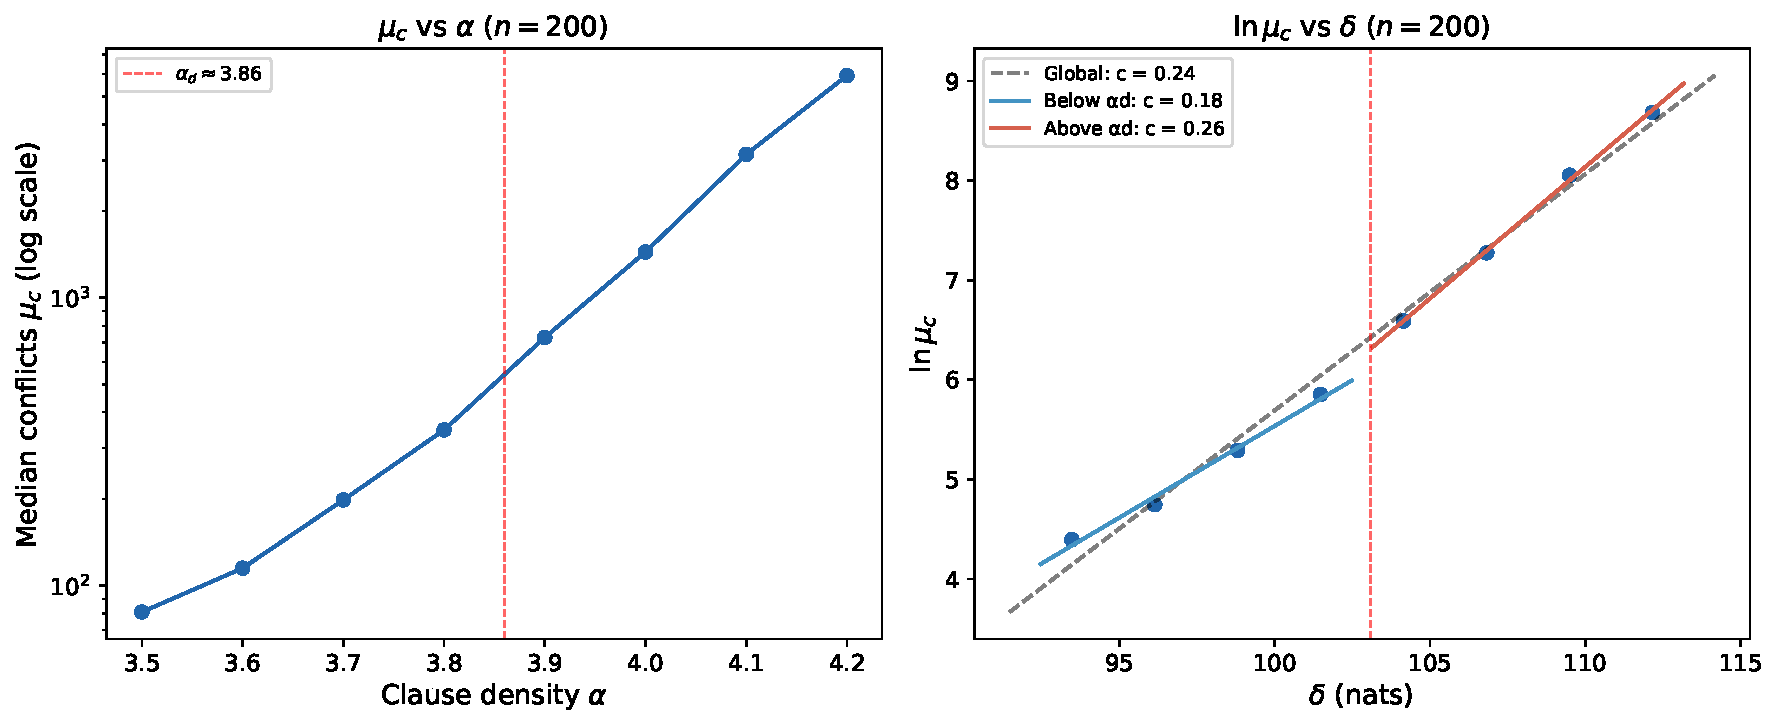
\includegraphics[width=\textwidth]{fig3_alpha_density.pdf}
\caption{Median CDCL runtime versus clause density ($n = 200$,
500~instances per~$\alpha$, $\alpha = 3.5$--$4.2$).
Left: $\mc$ on log scale.
Right: $\ln \mc$ vs~$\delta$ with piecewise linear fits
($c = 0.18$ below~$\alpha_d$, $c = 0.26$ above).
The vertical dashed line marks $\alpha_d \approx 3.86$.}
\label{fig:alpha_density}
\end{figure}


\section{Computational budget metrics}
\label{app:metrics}

\begin{table}[h]
\centering
\begin{tabular}{lcc}
\toprule
Metric & $c$ (CDCL) & $R^2$ \\
\midrule
Conflicts     & 0.194 & 0.991 \\
Propagations  & 0.082 & 0.757 \\
Decisions     & 0.040 & 0.488 \\
\bottomrule
\end{tabular}
\caption{Sensitivity exponent for different budget metrics ($n = 200$).
Conflicts yield the cleanest multiplicative separation,
consistent with conflicts representing the fundamental
state transitions of the CDCL algorithm.}
\label{tab:metrics}
\end{table}


%=============================================
% Bibliography
\begin{thebibliography}{15}

\bibitem{MPZ2009}
M.~M\'ezard, A.~Montanari,
\textit{Information, Physics, and Computation},
Oxford University Press, 2009.

\bibitem{Achlioptas2008}
D.~Achlioptas, A.~Coja-Oghlan,
``Algorithmic barriers from phase transitions,''
\textit{Proc.\ FOCS}, pp.~793--802, 2008.

\bibitem{Ding2015}
J.~Ding, A.~Sly, N.~Sun,
``Proof of the satisfiability conjecture for large $k$,''
\textit{Proc.\ STOC}, pp.~59--68, 2015.

\bibitem{Schoening1999}
T.~Sch\"oning,
``A probabilistic algorithm for $k$-SAT and constraint
satisfaction problems,''
\textit{Proc.\ FOCS}, pp.~410--414, 1999.

\bibitem{Gomes2000}
C.~P.~Gomes, B.~Selman, N.~Crato, H.~Kautz,
``Heavy-tailed phenomena in satisfiability and constraint
satisfaction problems,''
\textit{J.~Automated Reasoning}, 24(1/2):67--100, 2000.

\bibitem{Coarfa2003}
C.~Coarfa, D.~D.~Demopoulos, A.~San~Miguel~Aguirre, D.~Subramanian, M.~Y.~Vardi,
``Random 3-SAT: The plot thickens,''
\textit{Constraints}, 8(3):243--261, 2003.

\bibitem{MuHoos2015}
Z.~Mu, H.~H.~Hoos,
``On the empirical time complexity of random 3-SAT at the phase transition,''
\textit{Proc.\ IJCAI}, pp.~367--373, 2015.

\bibitem{Hoos1999}
H.~H.~Hoos, T.~St\"utzle,
``Towards a characterisation of the behaviour of stochastic local
search algorithms for SAT,''
\textit{Artificial Intelligence}, 112(1--2):213--232, 1999.

\bibitem{Frost1997}
D.~Frost, I.~Rish, L.~Vila,
``Summarizing CSP hardness with continuous probability distributions,''
\textit{Proc.\ AAAI}, pp.~327--333, 1997.

\bibitem{Aczel1966}
J.~Acz\'el,
\textit{Lectures on Functional Equations and Their Applications}.
Academic Press, 1966.

\bibitem{CoccoMonasson2001}
S.~Cocco, R.~Monasson,
``Trajectories in phase diagrams, growth processes, and
computational complexity: How search algorithms solve the
3-satisfiability problem,''
\textit{Physical Review Letters}, 86(8):1654--1657, 2001.

\bibitem{MarquesSilva1999}
J.~P.~Marques-Silva, K.~A.~Sakallah,
``GRASP: A search procedure for propositional satisfiability,''
\textit{IEEE Transactions on Computers}, 48(5):506--521, 1999.

\bibitem{SKC1994}
B.~Selman, H.~A.~Kautz, B.~Cohen,
``Noise strategies for improving local search,''
\textit{Proc.\ AAAI}, pp.~337--343, 1994.

\bibitem{BenSasson2001}
E.~Ben-Sasson, A.~Wigderson,
``Short proofs are narrow---resolution made simple,''
\textit{Journal of the ACM}, 48(2):149--169, 2001.

\bibitem{Pipatsrisawat2011}
K.~Pipatsrisawat, A.~Darwiche,
``On the power of clause-learning SAT solvers as resolution engines,''
\textit{Artificial Intelligence}, 175(2):512--525, 2011.

\end{thebibliography}

\end{document}
